\documentclass{article}
\usepackage{tikz}
\usetikzlibrary{lindenmayersystems} % LATEX and plain TEX when using TikZ
\begin{document}

\begin{tikzpicture}
\pgfdeclarelindenmayersystem{Koch curve}{
\rule{F -> F-F++F-F}
}
\shadedraw [top color=white, bottom color=blue!50, draw=blue!50!black]
[l-system={Koch curve, step=2pt, angle=60, axiom=F++F++F, order=3}]
lindenmayer system -- cycle;
\end{tikzpicture}

\pgfdeclarelindenmayersystem{Hilbert curve}{
\symbol{X}{\pgflsystemdrawforward}
\symbol{+}{\pgflsystemturnright} % Explicitly define + and - symbols.
\symbol{-}{\pgflsystemturnleft}
\rule{A -> +BX-AXA-XB+}
\rule{B -> -AX+BXB+XA-}
}
\tikz\draw[lindenmayer system={Hilbert curve, axiom=A, order=4, angle=90}]
lindenmayer system;

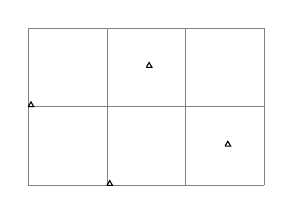
\begin{tikzpicture}
\draw [help lines] grid (3,2);
\pgfset{lindenmayer system/.cd, angle=60, step=2pt}
\foreach \x/\y in {0cm/1cm, 1.5cm/1.5cm, 2.5cm/0.5cm, 1cm/0cm}{
\pgftransformshift{\pgfqpoint{\x}{\y}}
\pgfpathmoveto{\pgfpointorigin}
\pgflindenmayersystem{Koch curve}{F++F++F}{2}
\pgfusepath{stroke}
}
\end{tikzpicture}

\tikz[rotate=65]\draw [green!60!black] l-system
[l-system={rule set={F -> F[+F]F[-F]}, axiom=F, order=4, angle=25,step=3pt}];

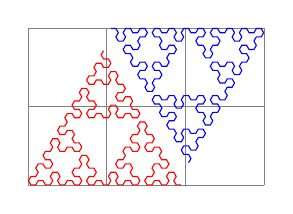
\begin{tikzpicture}[l-system={step=1.75pt, order=5, angle=60}]
\pgfdeclarelindenmayersystem{Sierpinski triangle}{
\symbol{X}{\pgflsystemdrawforward}
\symbol{Y}{\pgflsystemdrawforward}
\rule{X -> Y-X-Y}
\rule{Y -> X+Y+X}
}
\draw [help lines] grid (3,2);
\draw [red] (0,0) l-system
[l-system={Sierpinski triangle, axiom=+++X, anchor=south west}];
\draw [blue] (3,2) l-system
[l-system={Sierpinski triangle, axiom=X, anchor=north east}];
\end{tikzpicture}
\end{document}